\chapter{腰背痛}

腰背痛(low back
pain)一般是指定位于肋缘至臀皱褶下缘区域的疼痛、肌肉紧张或僵硬,伴或不伴有腿部疼痛(坐骨神经痛)。腰背痛是临床上最常见的症状之一。研究显示,约有80\%的人一生中会出现最少一次的腰背痛。大部分患者的腰背痛是由机械性因素所致,最常见的病因是随着年龄增长出现退行性变(椎间盘、椎骨)或反复的轻微损伤(包括肌肉、筋膜、韧带和神经)。90\%的腰背痛是一过性的,无需治疗在短期内可缓解,具有自限性;或通过一般物理治疗,在6周内缓解。部分腰背痛呈慢性反复发作过程,甚至可以影响患者生活和工作。临床上,多数腰背痛呈良性过程,但少数可以是机体有严重疾病的表现之一,包括感染、恶性肿瘤和其他系统性疾病。一般而言,严重破坏性病变引起的腰背痛并不常见。恶性肿瘤、感染、强直性脊柱炎和硬膜外脓肿引起腰背痛占到初级医疗单位就诊的全部腰背痛病例的比例不到1\%。然而,这些病因所致的腰背痛如果延误诊治,可能出现严重后果。因此,在腰背痛的鉴别诊断过程中,要特别注意排查这些疾病。

腰背部的解剖学结构包括有皮肤、皮下组织、筋膜、肌肉、韧带、椎骨、椎间盘、硬膜、脊髓和神经、大血管(主动脉和下腔静脉)、腹膜后组织或器官(肾脏、肾上腺、胰腺和淋巴结)以及腹腔或盆腔的内脏。这些组织和器官的病变均可引起腰背痛,因而腰背痛的病因可能非常复杂,有时不容易鉴别诊断。为了更好地进行定位诊断,可以将腰背痛按解剖部位分类为:脊椎疾病、脊椎旁软组织疾病、脊神经根及皮神经病损所致的腰背痛和内脏疾病所致的腰背痛。也可以根据腰背痛症状持续的时间,将腰背痛分为:急性腰背痛(<6周)、亚急性腰背痛(6~12周)和慢性腰背痛(>12周)。从病史上讲,一般急性腰背痛多与机械性因素有关,或者与破坏性病变导致的机械因素有关(如肿瘤侵蚀导致的骨折或压迫)。而慢性腰背痛则既与机械性因素有关,也可能与炎症性腰背痛或特异性的腰背痛有关。此外,还可以根据腰背痛发生的病因(表\ref{tab44-1}),将腰背痛分为:机械性腰背痛(机械性因素导致的腰背痛)、特异性腰背痛(由特定病因所导致的腰背痛)、内脏疾病牵涉的腰背痛和其他腰背痛(未知病因的腰背痛)。其中以机械性腰背痛最为常见,占所有腰背痛病例的90\%以上。病因分类可能更有助于指导治疗,故本章按病因进行论述。

应对腰背痛患者详细询问病史,认真进行体格检查,并根据病史和体检发现进行必要的辅助检查。

\begin{table}[htbp]
\centering
\caption{腰背痛的病因分类以及常见疾病}
\label{tab44-1}
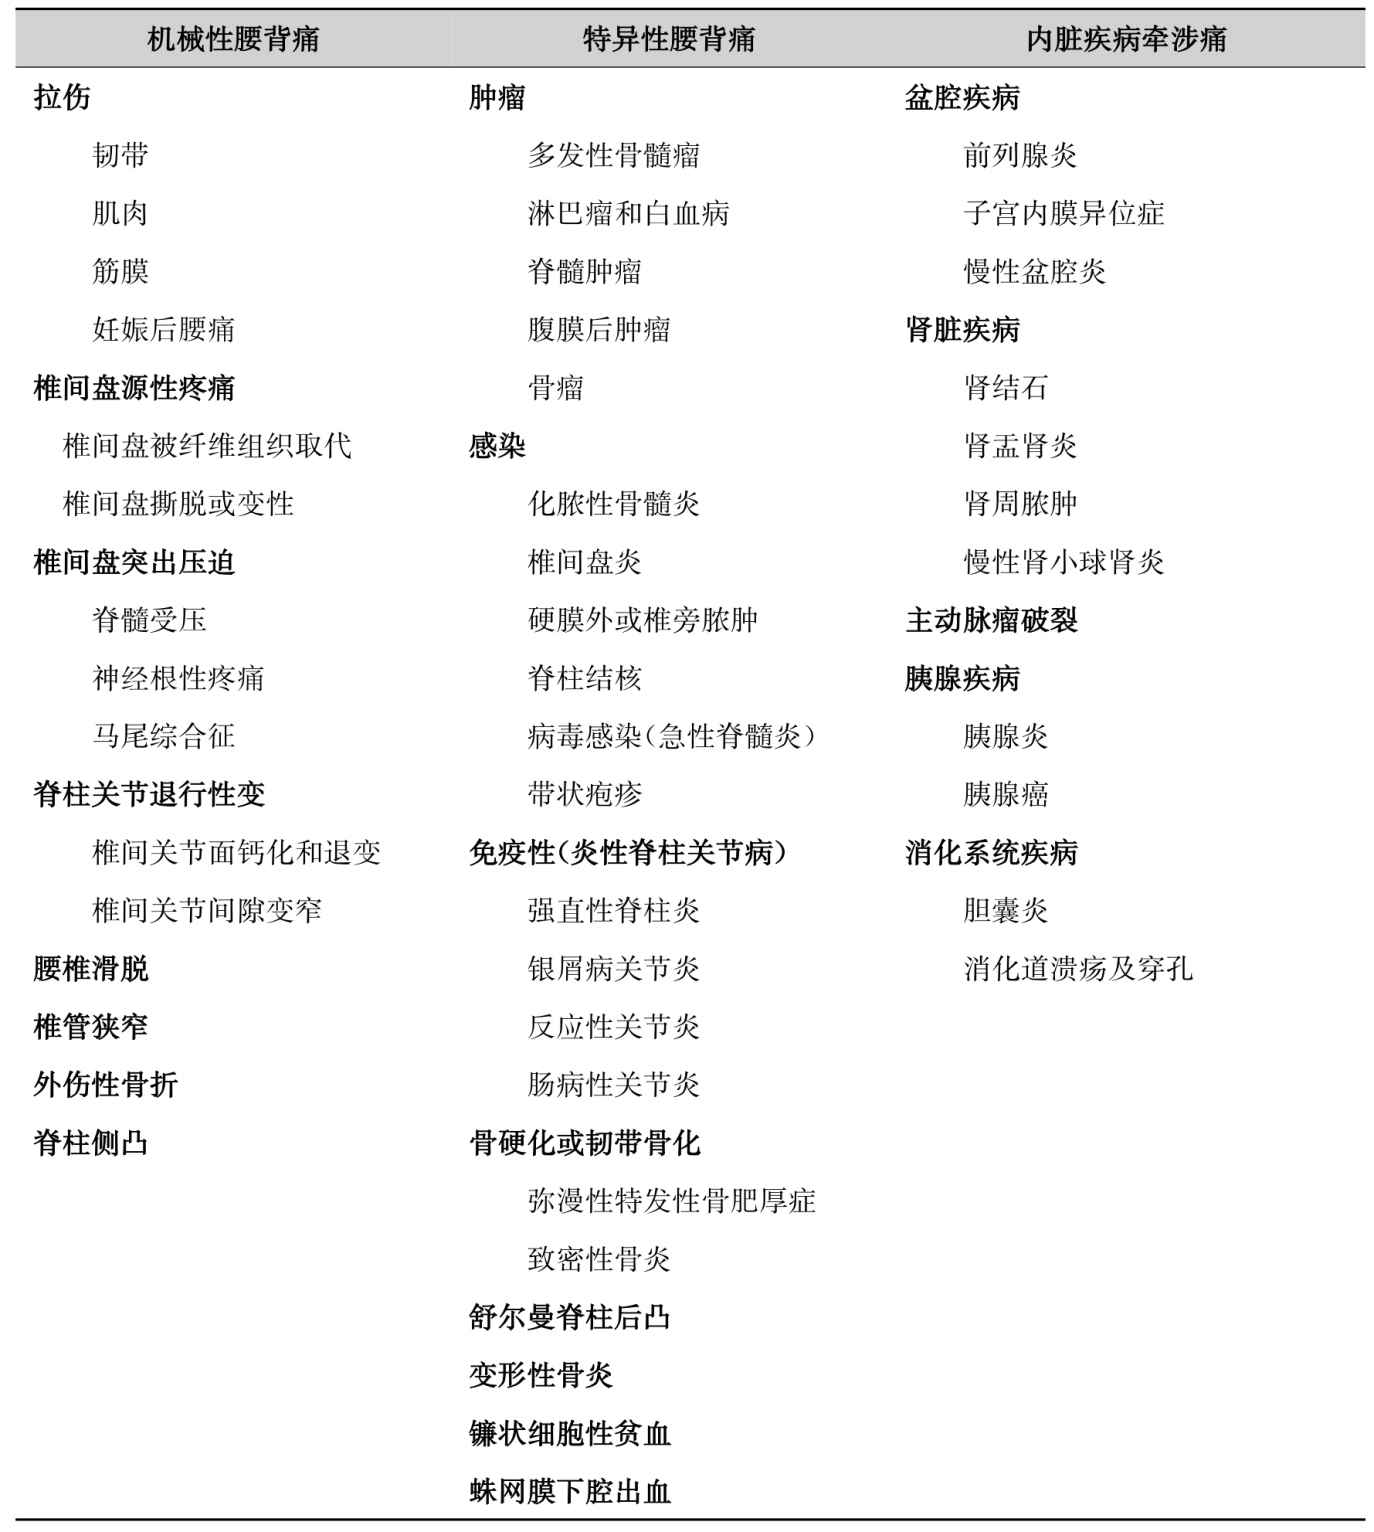
\includegraphics[width=5.91667in,height=6.60417in]{./images/Image00265.jpg}
\end{table}

\section{【病史采集】}

\subsection{(一)疼痛的特征}

注意了解腰背痛发生时的状况或诱因,包括疼痛的首发部位、疼痛的性质(跳痛、针扎样痛、烧灼样痛、酸痛)、程度(剧痛、钝痛、隐痛)、范围及分布、持续时间(一过性、持续性;疼痛持续时间<6周,6~12周,>12周)、缓解情况(休息或活动多久后改善)、加重的诱因(体位、站立、久坐、咳嗽、打喷嚏、深呼吸),有无放射痛(放射到臀部、膝以上、足部、会阴部)、伴随症状(大小便失禁、便秘、尿潴留、发热、盗汗、乏力、消瘦等)、有无神经系统表现(麻木、感觉异常、运动功能受损)以及疼痛对日常生活和睡眠的影响、对药物和物理治疗的疗效等。

\subsection{(二)有无严重疾病的危险因素}

了解患者从事的职业有助于腰背痛的诊断。一些抬、拉、推、扛重物、长期站立或行走的工种容易导致机械性的慢性腰背痛。研究发现:机械性腰背痛的危险因素包括:吸烟、肥胖、年龄、性别、体力劳动、久坐、工作压力大、文化水平低、对工作不满及心理因素如焦虑和抑郁。随着老年化趋势日益明显,骨质疏松引起的脆性骨折已经成为老年人腰背痛的主要病因之一。在询问病史时,应注意了解患者有无骨质疏松的危险因素,例如日照不足、维生素D或钙摄入不足(如乳制品摄入量少者可能钙摄入不足,脂肪吸收不良者容易出现维生素D缺乏)、体重轻、绝经早、有骨质疏松或脆性骨折家族史和长期使用糖皮质激素等。应注意寻找潜在疾病的危险因素,了解既往有无腰部手术史、有无肿瘤病史、有无心脏病史、有无咳嗽、血尿(肾绞痛)、尿潴留、尿失禁、下肢放射痛、神经系统异常。注意询问有无皮疹(银屑病,可致银屑病关节炎;带状疱疹在出现皮疹前也可能表现为腰背痛),有无慢性腹泻、便血(炎症性肠病可以出现肠病性关节炎),有无眼炎或视力突然下降(虹膜炎常常是脊柱关节病的一个关节外表现)、尿频-排尿不适、白带增多(泌尿生殖道感染可导致反应性关节炎)等。

出现下列情况提示可能存在潜在疾病:有肿瘤病史或结核病史、年龄大于50岁、不明原因消瘦、疼痛进行性加重、夜间痛、影响睡眠、对治疗无反应。吸毒、皮肤感染灶、持续发热或寒战、长期应用糖皮质激素或免疫抑制剂均应注意感染的可能(如结核)。对于40岁以下男性患者,若主要表现为腰背痛伴有晨起僵硬,特别是表现为夜间痛,活动后缓解,要考虑到患强直性脊柱炎的可能性。此外,还需注意排查内脏疾病,如十二指肠溃疡、胰腺炎、肾盂肾炎、主动脉瘤等其他严重的疾病引起的牵涉痛或放射痛。对于急性腰背痛,当存在危险因素时,需要进一步检查有无脊柱骨折、肿瘤、感染、马尾综合征。老年人需要注意有无骨质疏松症引起的压缩性骨折,年轻人一侧腰背痛要考虑有无椎体峡部骨折。有前列腺症状的患者,要考虑有无前列腺癌骨转移。

\subsection{(三)有无伴发神经受累的症状}

脊髓和神经根的病变常表现为腰背痛,询问病史应特别注意是否伴有神经受累的表现,常见的有坐骨神经痛、马尾综合征和椎管狭窄。坐骨神经痛的神经根受刺激最典型,呈剧烈刺痛或烧灼样痛,并放射到臀部和下肢侧面,甚至到足或踝部。疼痛放射到膝关节以下,更倾向于神经根性放射痛,而不是邻近的腿痛。坐骨神经痛往往伴有下肢麻木和刺痛,是由椎间盘突出压迫神经所致,在咳嗽、打喷嚏或深呼吸时症状加重。马尾综合征是马尾神经受到明显压迫时的表现,常由肿瘤或严重椎间盘膨出引起,可出现排便和排尿功能障碍,尿潴留常伴有充溢性尿失禁,并有会阴区麻木和下肢无力。椎管狭窄是由于椎管、神经根管、椎间孔狭窄而导致神经根受压,多由关节面增生性的骨赘、黄韧带增厚引起,椎间盘膨出和椎体滑脱也会导致椎管狭窄。椎管狭窄典型的症状包括:腰痛和下肢痛、坐位或弯腰时症状缓解。下肢有一过性的发麻或刺痛,行走时腓肠肌和下肢末梢疼痛加重,休息后缓解,称为神经性跛行。临床上需要通过检测动脉搏动情况来鉴别是否有血管闭塞引起的间歇性跛行。

\section{【体格检查】}

应根据病史采集所得,全面而有针对性地进行体格检查,以便对腰背痛进行定位和病因分析。进一步区别是内脏疾病牵引所致的腰背痛,如:胰腺炎、肾结石、动脉瘤;或是全身疾病所致,如结核、心内膜炎、镰状细胞性贫血或肿瘤;是否有局限性感染,如硬膜外脓肿、横贯性脊髓炎、骨髓炎、椎间盘炎等。还应重视神经系统检查,包括感觉和运动神经检查、坐位或卧位直腿抬高试验。了解是否有尿潴留,后者对诊断马尾综合征的敏感性高达90\%。同时还针对髂腰肌或肌腱、骶髂关节、梨状肌等部位进行相应的检查。

\subsection{(一)视诊}

体型是否对称,姿势,脊柱的生理弯曲,活动范围,肌肉分布是否对称,有无皮疹,左右髂骨是否在同一水平线上(用于判断双腿是否等长),脊柱活动度,步态,行为(呻吟、行动缓慢、手支撑腰部)。踮脚尖走路(S\textsubscript{1}
),踮脚后跟走路(L\textsubscript{5}
),原地踏步、蹲下起立,单腿直立。宽基步态提示脊髓病变。手支撑步态提示L\textsubscript{2}
~L\textsubscript{4}
节段引起股四头肌无力。足下垂或跨步步态提示L\textsubscript{4}
~L\textsubscript{5} 节段病变。平足或足不能蹬地提示S\textsubscript{1}
~S\textsubscript{2}
节段病损引起腓肠肌、比目鱼肌无力。鸭步提示髋关节病变,或L\textsubscript{5}
支配的臀中肌无力。通过观察姿势可以发现局限性疼痛、肌肉痉挛或畸形的部位,以及患者站立时脊柱后凸、前凸、侧凸的方向和部位。

\subsection{(二)触诊}

了解椎旁肌肉对称性,有无触痛、肌肉痉挛和肿块,腰扭伤常有椎旁肌肉痉挛、触痛,多个腰椎节段运动时疼痛加重。检查是否有棘突叩痛,分清触痛是来自于椎体还是软组织。椎体触痛敏感,但不特异,在脊髓感染时比较敏感特异。老年人行走时出现腓肠肌疼痛,应检查外周血管搏动,对判断血管性跛行或是神经性跛行有意义。有腿部症状的患者要进行直腿抬高试验和L\textsubscript{5}
和S\textsubscript{1}
神经根的检查。直腿抬高试验对鉴别神经根病疼痛有帮助:患者处于仰卧位,检查者抬起患者的腿部,踝部背曲,患者完全放松不用力支持,当大腿抬高到10°~60°范围引起坐骨神经痛,即为阳性。交叉直腿抬高试验:抬高没有疼痛的一侧下肢,如果出现对侧受累的下肢再次出现疼痛即为阳性。坐位直腿抬高试验:患者坐位,缓慢抬高下肢,当髋关节屈曲90°时,出现坐骨神经痛的症状即为阳性。直腿抬高试验对椎间盘突出敏感,特异性差,交叉直腿抬高试验对椎间盘突出症特异度高。存在持续的疼痛应进行系统的体格检查和肿瘤相关检查包括乳房、前列腺、淋巴结检查。

精神因素可以影响疼痛的发生,为排除精神因素的影响,可以进行捏脊试验、扭转试验、头部压迫试验或坐位直腿抬高试验。具体做法,捏脊试验:站位或俯卧位时卷压患者背部松弛皮肤,询问患者有无神经根症状产生,正常情况下不出现神经根症状。扭转试验:患者站立位,检查者用手扭转患者躯干。这样可以引起脊柱活动,但全部的转动发生在膝关节,因而不会产生背部疼痛。头部压迫试验:在头顶使用大约2公斤的力量下压,这一重量并不足以引起机械性疼痛或不稳。坐位直腿抬高试验:仰卧位时直腿抬高试验出现症状,而坐位时无症状为假阳性。正常情况下,若果有神经根压迫,坐位直腿抬高加重坐骨神经根疼痛症状,身体后倾以避免疼痛加重。

\subsection{(三)神经系统检查}

对怀疑有神经根和脊髓受累的患者,应行神经系统检查,包括感觉、肌力和反射三方面。

\subsubsection{1.感觉的检查}

包括触觉、针刺痛觉、振动觉、本体感觉、温度觉、疼痛反应,根据感觉平面来判断脊髓损伤平面。体表标志,T\textsubscript{4}
感觉支配区位于胸壁乳头平面,T\textsubscript{7}
感觉支配区位于剑突以及胸骨下部,T\textsubscript{10}
感觉支配区位于腹壁脐平面。腰椎神经感觉平面位于下肢,沿大腿及小腿斜形分布。L\textsubscript{2}
支配大腿前部,L\textsubscript{3} 支配膝关节前方,L\textsubscript{4}
~S\textsubscript{1} 在足部检查,L\textsubscript{4}
支配足内侧,L\textsubscript{5} 支配足背,S\textsubscript{1}
支配足外侧。骶神经支配会阴区的皮肤感觉,形成以S\textsubscript{5}
为中心的肛周环形感觉支配区。会阴部感觉检查最好与肛门反射及球海绵体肌反射(阴茎)反射配合。

\subsubsection{2.肌力检查}

L\textsubscript{1} ~L\textsubscript{2}
检查髋关节屈曲,L\textsubscript{3} 检查伸膝功能,L\textsubscript{4}
检查胫前肌伸踝关节功能,L\textsubscript{5}
检查
\includegraphics{./images/Image00266.jpg}
长伸肌伸
\includegraphics{./images/Image00267.jpg}
趾功能。S\textsubscript{1} 检查腓肠肌跖屈踝关节功能。

\subsubsection{3.反射检查}

T\textsubscript{7} -L\textsubscript{1}
对应腹壁浅反射检查,L\textsubscript{4}
对应膝反射检查,S\textsubscript{1}
对应跟腱反射和踝反射,有无巴宾斯基征(Babinski)。

98\%的椎间盘突出发生在L\textsubscript{4} ~L\textsubscript{5}
和L\textsubscript{5} ~S\textsubscript{1}
,因此,神经系统检查主要应针对L\textsubscript{5} 和S\textsubscript{1}
神经根检查(表\ref{tab44-2})。L\textsubscript{5}
神经根运动检查包括:踝和大
\includegraphics{./images/Image00268.jpg}
趾背屈的力度。L\textsubscript{5}
神经根感觉检查包括:足内侧的麻木感、第一二足趾间感觉。S\textsubscript{1}
神经根主要判断踝反射和腓肠肌和足侧感觉,S\textsubscript{1}
神经根受损可出现跖屈无力,可以让患者踮脚尖走路来判断。尽管踝反射在S\textsubscript{1}
神经根受累检查中是很重要的,但随着年龄增长,踝反射逐渐减弱,一般是双侧同时减弱。因此,单侧踝反射减弱对神经根受损的判断还是有临床价值的。在慢性疼痛的患者中,精神因素会让人认为疼痛明显,并且伴有不真实的体征,表面皮肤的触痛,坐位和仰卧位直腿抬高试验阳性结果不一致,在体格检查中反应敏感,这些称为Waddell征。

\begin{table}[htbp]
\centering
\caption{神经根受压的神经系统体格检查}
\label{tab44-2}
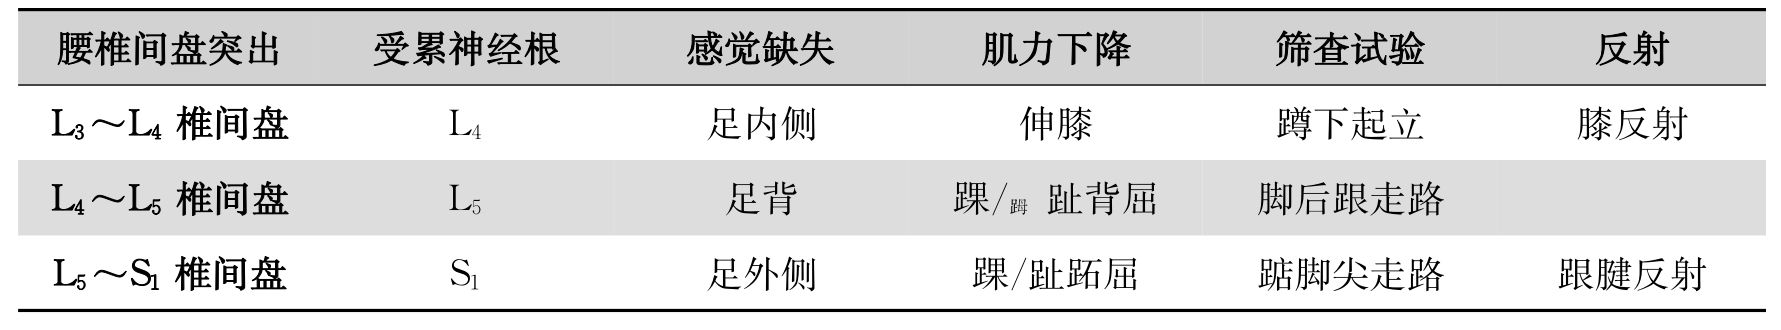
\includegraphics[width=5.92708in,height=1.08333in]{./images/Image00269.jpg}
\end{table}

\section{【实验室检查】}

大部分腰背痛患者实验室检查均为阴性,特别是机械性腰背痛患者的血清炎症指标多为正常,但炎性腰背痛患者血红细胞沉降率(血沉)测定和C反应蛋白(CRP)常升高。血沉和CRP的检测有助于鉴别炎症性和机械性腰背痛。细菌感染所导致的腰背痛(如化脓性脊椎炎)ESR和CRP均升高,同时伴有细菌感染的其他表现如血白细胞升高、核左移,血清降钙素原水平升高。肿瘤所致的腰背痛,血沉常增高,但CRP升高不显著(淋巴瘤除外)。对于自身免疫相关的腰背痛如强直性脊柱炎,患者的血沉和CRP均升高,但血清降钙素原水平正常;患者常有HLA-B27阳性,有助于诊断。免疫抑制的高危人群需要做结核菌素试验。伴有高热、发冷或寒战者,应做血、尿、痰或静脉置管的可疑病原体培养。怀疑脊柱多发性骨髓瘤时,应进行尿本周蛋白测定和血清蛋白固定电泳,这些检查对该病诊断很有意义。

\section{【影像学检查】}

\subsection{1.X线平片}

广泛应用于了解骨骼结构,具有简便和价格便宜的优点,但普通X线摄片对于软组织显像能力有限,仅可以发现肿胀、局部包块、积气以及不透射线的异物。尽管其分辨率低,但对于脊柱病变仍是首选的影像学检查方法。X线摄片检查比较容易发现的骨骼和关节病变包括脊柱畸形、骨质疏松、椎体骨折、椎体骨质增生、椎间盘变窄、韧带钙化、关节侵蚀(特别是骶髂关节)、关节融合、脊柱强直等。

\subsection{2.CT检查}

CT检查虽然比普通X线摄片昂贵,但可以获得躯体断层图像,而且分辨率大大高于普通X线摄片,是腰背痛鉴别诊断的重要检查手段,尤其适合于结构复杂部位(如脊柱和骨盆)的检查。CT对软组织分辨率不如磁共振(MRI)检查,但对骨关节的检查分辨率却高于MRI,因而特别适用于脊柱创伤的检查,可用于明确是否有骨块向后移位造成的椎管狭窄以及脊柱后方结构是否有骨折。通过数据处理和重建还可以获得三维图像,以便医师进行立体图像分析。

\subsection{3.磁共振(MRI)检查}

MRI具有非侵袭性、非放射性以及多维分析能力的特点,对软组织的分辨率比其他检查手段高,缺点是检查时间较长、价格贵,而且植入金属可以产生伪影而影响成像。MRI在脊柱和骶髂关节疾病的诊断中具有非常重要的价值。正常成人骨髓由于脂肪含量较多,因而在T1加权像和T2加权像上显示高信号。椎间盘在T1加权像上为低信号,在T2加权像上为高信号。通过采用抑制脂肪显像(压脂序列)T2加权像,能很好地显示水分,因而能很好地显示骨髓或软组织是否有炎症水肿。虽然MRI对骨的显像不如CT,但对骨创伤、骨髓炎和脊柱关节病中的骨髓水肿能很好地显示,从而对诊断骨和软组织的炎症,具有很高的敏感性。对于脊柱肿瘤,MRI检查更为敏感准确。

\subsection{4.放射性核素扫描(ECT)骨显像}

锝标记的骨显像检查在骨科影像学检查中扮演重要角色。多用于检查脊柱有无转移性病灶,识别应力性骨折和骨髓炎。ECT检查可以显示骨的代谢活动情况,但特异性低。

90\%的腰痛可逐渐缓解,没有必要对所有患者进行影像学检查,尤其是对年轻女性,保护其性腺功能,避免过多进行腰椎和胸部X线检查。一般在疼痛发生的前4~6周不建议做相关影像学检查,而且先进的影像技术如MRI在提高敏感性的同时也增加了假阳性机会,容易增加患者焦虑,导致过度治疗。不过,临床上若存在提示严重疾病的信号则需要及时进行影像学检查,以尽早明确诊断和及时治疗。这些危险信号包括:进行性加重的神经系统症状和体征,伴随明显的全身症状,发病时有外伤史,有恶性肿瘤病史,年龄大于50岁,或起病年龄小并持续存在的炎性腰背痛(夜间痛、活动后减轻),有感染因素存在(吸毒史、使用免疫抑制剂、停留导尿管、长期应用糖皮质激素、皮肤或泌尿系感染),骨质疏松症,出现马尾综合征表现(典型的尿潴留和排便困难,会阴区麻木、双下肢无力或麻木),脊髓压迫(急性神经功能缺失,可以是肿瘤或脊髓转移瘤导致),持续性坐骨神经痛,感觉缺失,反射减弱,直腿抬高试验阳性以及运动神经受损等。

在临床症状持续4~6周无缓解的情况下,宜行腰椎前后位片和侧位片,排除肿瘤、感染、腰椎不稳、脊柱关节病和腰椎滑脱;腰骶部疼痛还需做骨盆照片,了解骶髂关节情况。在肿瘤和感染的鉴别诊断中,CT和MRI检查要优于X线检查,对椎间盘突出和椎骨狭窄也十分有价值,但不推荐患者疼痛早期频繁的做这些检查。若高度怀疑肿瘤和感染,则应及时进行CT
或MRI检查。

\protect\hypertarget{text00333.html}{}{}

\section{145 机械性腰背痛}

\subsection{一、腰肌劳损或扭伤}

\subsubsection{(一)急性腰扭伤}

急性腰扭伤常有明确的腰部扭、闪和挫等外伤史,其特点伤后立刻出现腰或骶部剧烈疼痛,但有时次日才出现疼痛。主要表现为活动困难,腰部弯曲、活动或咳嗽、深呼吸动作疼痛加重。查体:身体姿势固定,活动或翻身困难,常用手撑住腰部。腰椎椎旁肌肉痉挛僵硬,脊柱向患侧倾斜。有明显的浅表性压痛点。X线无异常改变。

\subsubsection{(二)腰背部肌筋膜炎(腰肌劳损)}

多见于青壮年,有时外伤史不明显,常与职业和工作环境有一定的关系。表现为腰背部酸痛或胀痛,适当活动或经常改变体位症状可减轻。缓慢发病,受凉或劳累后加重,休息后缓解。有时在髂嵴上、骶髂肌或腰方肌上可触及局限性结节。X线无异常。

\subsubsection{(三)梨状肌损伤综合征}

梨状肌损伤综合征好发于女性。梨状肌为臀部深层的一块形似梨形的小肌肉,它起于骨盆内骶骨前面2、3、4骶前孔的外侧,向外下穿过坐骨大孔到臀部,以肌腱止于股骨大粗隆的后内侧,是髋关节的外旋肌。由于梨状肌的下方有坐骨神经通过,当梨状肌紧张、痉挛,造成局部组织充血、水肿和挛缩时,刺激或挤压坐骨神经,从而产生坐骨神经压迫症状,出现腰腿疼痛,临床表现类似坐骨神经痛。梨状肌损伤综合征的病因尚不明确,其发生可能与梨状肌损伤有关,急性损伤者疼痛明显,患肢可有跛行。慢性损伤者感患侧臀部或下肢酸胀麻痛。查体:直腿抬高试验在60°以前臀部及下肢疼痛剧烈,但当超过60°时疼痛反而减轻(梨状肌不再被牵拉),梨状肌紧张试验阳性。经肛门或阴道检查若发现梨状肌触痛有助于诊断。X线检查无异常,但有时MRI检查可以发现肌肉水肿。

\subsubsection{(四)妊娠期骶髂关节痛}

在妊娠的最后几个月,骶髂关节的支持韧带变得松弛,孕妇可以发生骶髂关节处疼痛,可放射到大转子并向下放射到大腿前内侧。

\subsection{二、退行性疾病}

\subsubsection{(一)胸椎退行性变}

脊椎退行性病变是中老年人腰背痛的主要病因之一,胸椎及椎间盘病退行性变,可引起椎骨增生、骨赘形成、黄韧带肥厚、椎管及椎间孔变形狭窄或椎间盘突出,引起相应的神经根或脊髓压迫症状。疼痛是最常见的症状,可能伴有运动和感觉障碍。疼痛表现为轴性或根性。根性疼痛表现为胸部或腹部的束带状疼痛。症状部位与病变节段有关,大部分患者表现在T\textsubscript{10}
节段症状。感觉迟钝比感觉缺失更为常见。尤其注意有腱无反射异常,下肢腱反射亢进而上肢检查正常,表明胸段脊髓受压。其他表现还包括:步态不稳、踝阵挛、巴宾斯基征阳性。X线表现有:椎体出现骨赘、椎间隙变窄及小关节突肥大。CT扫描可显示骨质增生或后纵韧带骨化、椎间盘突出。MRI检查可见脊髓受压现象。无症状患者出现影像学异常的表现发生率高,因此MRI可能会过度诊断椎间盘突出。

\subsubsection{(二)腰椎退行性变}

腰椎退行性变包括:腰椎间盘纤维环、椎间盘髓核、软骨终板、腰椎体、腰椎小关节、黄韧带和椎管的退行性变及骨赘形成。退行性变通常见于老年人,无性别差异,表现为下腰痛以及逐渐加重的腿痛。腰部或臀部的钝痛或锐痛,可放射至大腿或小腿,行走或活动时可引起典型的下肢疼痛、麻木、无力、感觉异常,称为神经源性跛行。必须和血管源性跛行相鉴别。血管源性跛行常出现在夜间,可以痛醒,把腿从床边垂下可减轻疼痛,前倾姿态难以减轻小腿疼痛,外周血管搏动通常会减弱或消失,小腿伴有烧灼样疼痛。相反神经源性疼痛通常向前弯腰可以缓解,行走时推购物车可以缓解疼痛,上坡比下坡引起的疼痛轻,停止活动后疼痛缓解快。小腿产生刺痛、麻木和无力的症状。

\subsubsection{(三)退行性腰椎滑脱}

主要发生在40岁以后的成年人,与关节突小关节和腰椎间盘退变有关。L\textsubscript{4}
~L\textsubscript{5}
最常见,女性多于男性。临床表现为典型的下腰痛,向下放射至臀部和大腿外侧,行走后出现无力,下肢沉重感,以及间歇性跛行。有一半以上患者出现根性疼痛,L\textsubscript{5}
神经根症状明显。马尾综合征很少出现,但随着病程进展,开始出现尿等待、尿不尽以及控制无力等症状。这些症状常被误认为是老年性泌尿系统常见的现象。X线检查应该进行立位侧位照片,卧位照片容易漏诊。CT具有较好的诊断价值。MRI可看到神经根压迫、椎间盘退变、小关节滑囊囊肿、黄韧带肥厚及其他压迫神经根的软组织。

\subsubsection{(四)腰椎间盘突出}

椎间盘突出分类:①膨出型:纤维环完整,椎间盘环形膨隆;②突出型:突破纤维环但仍和残余髓核连续;③游离型:髓核丧失完整性(游离碎片);④包含型:韧带下(后纵韧带下或外层纤维环下);⑤未包含型:穿过后纵韧带或外层纤维环。

椎间盘突出典型的症状是腰痛伴有根性疼痛。腰痛是最先出现的症状,有时可伴有臀部疼痛。常有摔倒、扭伤和提重物等诱因。下腰椎和腰骶段的椎间盘突出可以引起典型的放射至膝关节以下部位疼痛。高位椎间盘突出(L\textsubscript{2}
~L\textsubscript{3} 、L\textsubscript{3} ~L\textsubscript{4}
)可以引起股神经痛,但临床少见,不足5\%。绝大多数患者是L\textsubscript{4}
~L\textsubscript{5} 和L\textsubscript{5} ~S\textsubscript{1}
椎间盘突出,表现为坐骨神经痛,典型的坐骨神经痛是从下腰部向臀部、大腿后方、小腿外侧直到足部的放射痛,打喷嚏和咳嗽等腹压增高的情况下疼痛加剧。L\textsubscript{1}
可引起腹股沟疼痛,L\textsubscript{2} 和L\textsubscript{3}
神经根病变可引起大腿中部或腹股沟疼痛,L\textsubscript{5}
神经根疼痛可导致足背部出现症状。S\textsubscript{1}
可放射到腓肠肌后部和足底趾部。马尾综合征最常见于腰椎间盘突出症,L\textsubscript{4}
~L\textsubscript{5}
椎间盘最常受累,为外科急症,主要包括会阴部感觉障碍(鞍区麻痹),大小便障碍,新发的下肢感觉障碍,进行性运动功能障碍(表\ref{tab44-3})。体格检查注意观察患者步态,坐骨神经痛患者表现腰椎侧凸,躯体向健侧弯曲。腰椎活动受限,尤其是急性期,前屈受限明显。椎旁肌肉痉挛,椎体压痛。仰卧位进行直腿抬高试验,当抬至35°~70°时出现坐骨神经痛为阳性。直腿抬高试验对于检查L\textsubscript{4}
、L\textsubscript{5} 和S\textsubscript{1}
神经根病变最敏感,而交叉直腿抬高试验时,抬高健肢时患者主诉患肢疼痛,在腰椎间盘突出症的诊断中具有特殊意义,此体征对确诊很有价值。Lasegue征:当足部背屈时,加重疼痛为直腿抬高加强试验阳性。股神经牵拉试验:患者俯卧位,抬高对侧下肢时出现同侧疼痛症状为阳性。视受累脊神经根的部位不同而出现该神经支配区感觉异常。早期表现为感觉过敏,渐而出现麻木、刺痛及感觉减退。大部分患者出现肌力下降,L\textsubscript{5}
神经根受累时,表现踝及趾背伸肌力下降,S\textsubscript{1}
神经根受累时,表现趾及足跖屈肌力下降。足下垂或者足拖行与L\textsubscript{4}
~L\textsubscript{5}
神经根麻痹有关。X线不能显示椎间盘突出,可显示脊柱侧凸、椎间盘钙化、骨赘形成、椎间隙变窄、椎体间轻微滑脱、关节突关节肥大及矢状面序列的变化。CT可较清楚地显示椎间盘突出的部位、大小、形态和神经根、硬脊膜受压移位的情况,同时显示椎板及黄韧带肥厚、小关节增生肥大、椎管及侧隐窝狭窄等情况。MRI能够清楚地区分游离型与突出型椎间盘突出。

\begin{table}[htbp]
\centering
\caption{马尾综合征和脊髓压迫鉴别特点}
\label{tab44-3}
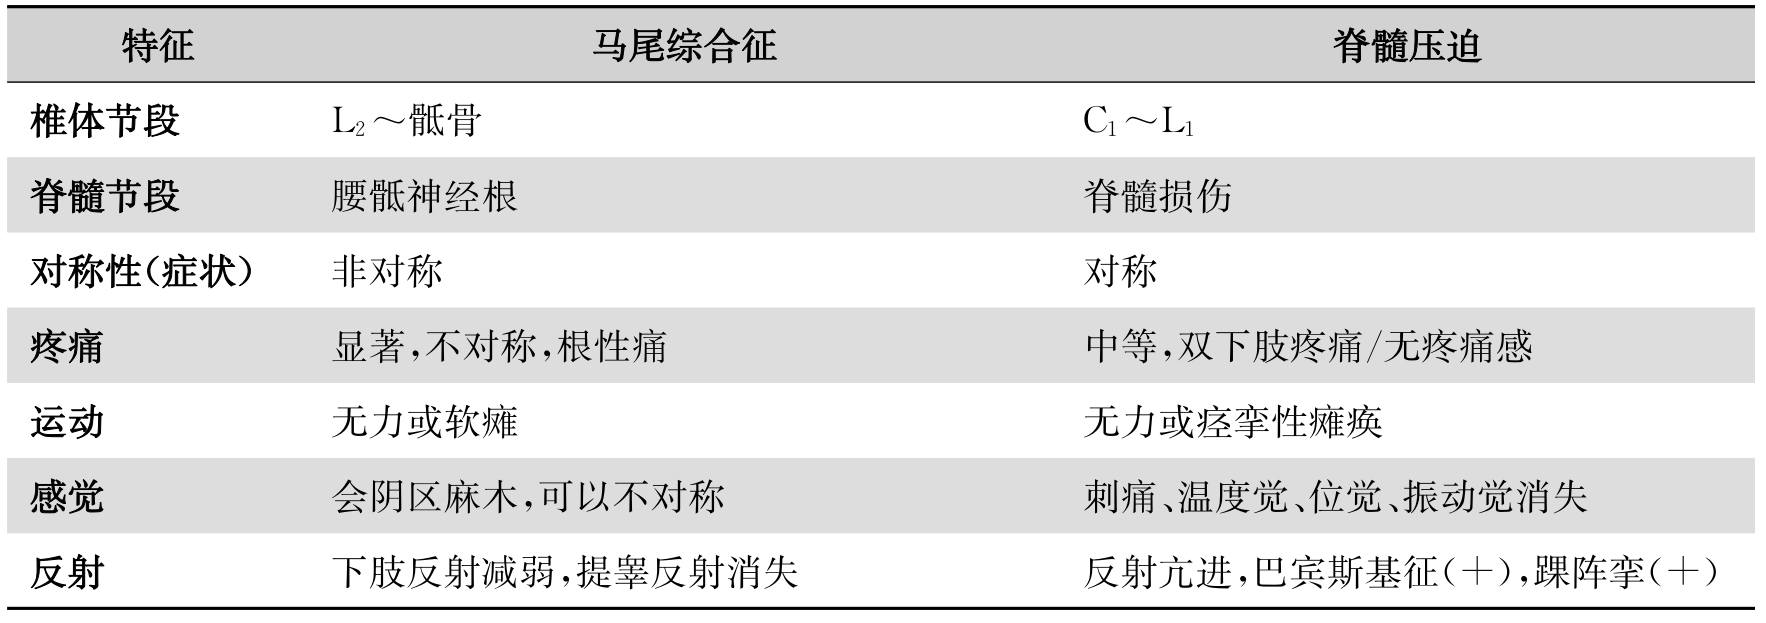
\includegraphics[width=5.875in,height=2.07292in]{./images/Image00270.jpg}
\end{table}

\subsection{三、先天性脊柱畸形}

先天性脊柱侧凸 从患者的出生史、发育史、家族史到完整的系统检查是该病诊断的依据。先天性脊柱畸形中,有33\%患者合并泌尿生殖系统畸形,25\%患者出现颈椎融合,10\%患者合并先天性心脏病。体格检查中可见头部偏斜或身体中线偏移,旋转状肋骨隆凸,或躯干矢状面畸形,还有一些特殊表现,包括背部皮肤多毛斑、皮肤凹陷、包块、痣、脂肪瘤等。下肢畸形足、高脚弓内翻足、下肢肌肉萎缩、双侧反射不对称、双下肢不等长等。

\subsection{四、外伤性骨折}

脊椎骨折的患者多为青壮年体力劳动者,常因由高空跌下,足部或臀部首先着地,脊柱突然过度前屈,而发生脊椎压缩性楔形骨折;又如固定物从高处冲击肩部或背部以及抬重物时失足滑倒,均可发生椎体压缩性骨折。此类屈曲型脊柱骨折最常见,占脊椎骨折病例的90\%,最常发生于第11~12胸椎和第1、2腰椎。另一种情况是患者从高空仰面落下,腰和背先着地,使脊柱过分后伸,发生伸直型脊椎骨折,此类骨折极少见。诊断脊椎骨折主要根据以下几点:①有明确的外伤史;②骨折部位压叩痛,脊柱可有后凸或侧凸畸形,活动障碍,肌肉痉挛,可表现为腹肌紧张而误诊为急腹症,少有局部血肿,严重者特别是合并脱位时,常并发不同程度的脊髓神经损伤,如胸或腰段脊柱骨折出现骨折部位以下截瘫;③X线检查是诊断本病最可靠的方法,对疑似病例作正、侧位X线摄片检查,即可发现有无骨折或脱位。

脊椎骨折和脱位如在畸形状态愈合,可产生损伤性关节炎,以及负重力线改变而出现自发性腰背疼痛和脊柱活动障碍。

\protect\hypertarget{text00334.html}{}{}

\section{146 特异性脊柱病变}

\subsection{一、感染性脊柱炎}

\subsubsection{(一)化脓性脊柱炎}

化脓性脊柱炎是由细菌感染所导致的脊柱感染,可由血源性播散或直接播散引起,致病菌以金黄色葡萄球菌多见。最常见的播散途径是血源性播散,包括泌尿系统、呼吸系统和皮肤感染。医源性的病因,如留置导尿管、脊柱手术或脊柱内注射侵入性的操作。化脓性脊柱感染的危险因素包括酗酒、糖尿病、其他部位感染、艾滋病、免疫抑制、留置导尿管、静脉吸毒、男性、恶性肿瘤、营养不良、病态肥胖症、脊柱手术操作、慢性肾脏疾病、类风湿关节炎、皮肤感染、吸烟、创伤等。过半患者可以找到感染源,腰椎比颈、胸椎更多见。儿童多出现椎间盘炎,成人多出现化脓性骨髓炎。腰背痛是成人脊柱感染最常见主诉,疼痛症状有时不典型。大多数起病隐匿,一半患者在发病3个月后确诊。疼痛性质为持续性后背痛,负重时疼痛加重。通常累及邻近的两个椎节和椎间隙。椎体破坏和塌陷程度不一,伴有脓肿,向前或向后扩散,出现神经刺激征和脊髓压迫征。疼痛常常伴有发热、盗汗、寒战、消瘦等。经常会出现椎旁肌肉痉挛和受累脊柱节段因疼痛引起活动受限。邻近腰大肌受累时,疼痛引起髋关节异常。神经根症状相对少见,但出现硬膜外脓肿压迫时,神经系统症状明显。儿童症状特殊,婴儿和刚学步的幼儿症状明显,表现行走困难,甚至拒绝行走。大龄儿童主诉腹痛或腰背痛,表现为脊柱强直和局限轻压痛。脊柱僵直,棘突压痛,叩诊时腰背痛加重,当合并硬膜外脓肿穿孔时,可直接压迫或损伤导致脊髓下段和马尾损伤。只有三分之一患者白细胞计数异常,ESR、CRP对脊柱感染敏感,但不特异。有体温波动,怀疑脊柱感染的患者均应行血培养。X线在早期感染无阳性表现,在12周后出现变化。X线可见椎间隙变窄,相邻椎体终板的骨质破坏,反应性骨增生、骨硬化。MRI是最具诊断价值的影像学方法,可显示椎间盘、硬膜外间隙和椎旁组织的解剖结构异常,可见椎旁脓肿和硬膜外脓肿。在感染的椎体或椎间盘中,由于炎症和水肿出现,T1加权像信号强度减低,T2加权像高信号,造影剂增强MRI对硬膜外脓肿更敏感。CT评估溶骨性缺损,当MRI有禁忌时可采用ECT检查。

\subsubsection{(二)脊柱结核(Pott病)}

脊柱结核好发20~30岁成人,艾滋病患者发病率较高。本病多发生在下胸椎和上腰椎,常位于椎体,不易破坏椎间盘,在前纵韧带的后方上下蔓延。结核发病隐匿,可长达半年。幼儿容易激惹,不敢坐及行走。青少年和成人表现单纯的腰背痛。早期出现局限性腰背部疼痛,肌肉痉挛,活动受限,神经刺激征和脊髓压迫征,常出现腰背痛和局限性后凸,刺激神经根,可引起肋间神经痛。一侧或两侧腰大肌脓肿,脓肿多位于椎旁,刺激神经根,引起刺激性疼痛。截瘫是脊柱结核最常见的神经功能障碍。可伴有间歇性发热、盗汗、厌食、乏力、体重下降等结核中毒症状。查体:脊柱僵硬,因局限性椎体破坏塌陷导致脊柱后凸畸形。腰椎结核表现为下腰痛,活动受限,棘突压痛和叩击痛阳性,拾物实验阳性。脊髓受压迫后出现截瘫的各种体征。实验室检查包括贫血、低蛋白血症、ESR和CRP升高,PPD试验阳性。X线上表现,早期侵及椎体前面,逐渐向后蔓延至整个椎体和椎间盘,胸椎后凸增加,椎体骨质破坏,空洞,死骨形成,椎间隙狭窄或消失,椎旁阴影增宽。多个椎体感染、破坏导致椎体前缘呈扇贝形。CT比X线出现的表现要早,可发现骨碎片、溶骨性改变、局限性硬化和骨膜下反应。冷脓肿中可见钙化及软组织中的骨碎片。CT还可以引导穿刺活检。MRI能发现椎体内或椎旁脓肿,对脊髓结核诊断意义更大。

\subsubsection{(三)梅毒性脊椎炎}

夏科(Charcot)关节病是脊柱梅毒感染最常见的表现,好发于胸腰段,出现破坏和肥大性改变。脊椎完全塌陷时可发生脊髓或马尾横断性损伤。脊柱改变以严重肥大性脊柱炎、增生、大量骨赘、椎间隙消失或狭窄为特点。血清梅毒试验阳性。

\subsubsection{(四)布鲁菌性脊椎炎}

多见于男性农牧民和毛皮加工者,有腰背部疼痛,急性期伴有发热,寒战,血清布氏杆菌凝集试验阳性。X线可见骨质破坏、关节间隙变窄、椎体骨质增生、硬化,椎旁脓肿少见,多发生在下腰椎,脓肿主要位于受累椎间盘周围。

\subsubsection{(五)脊柱包囊虫病}

牧区农民多见,有狗、羊接触史,X线可见椎体囊性破坏,并有椎体膨大或病理性骨折,包囊突向椎体两侧,形成假性椎旁脓肿,椎板及关节突等部分亦可有囊性破坏区。实验室检查嗜酸性粒细胞计数增多,包虫皮试(Casoni试验)阳性。

\subsubsection{(六)真菌性脊椎炎}

真菌感染多伴球孢子菌和芽生菌感染,是播散性疾病的一部分,椎体活检可以明确诊断。

\subsubsection{(七)带状疱疹}

带状疱疹在出现皮疹前,可以表现为腰痛或腹痛,多为刺痛或电击样痛,因没有疱疹或仅有细小的皮疹,故容易漏诊,等到带状排列的疱疹出现之后才确诊。因而在腰痛的体检中,应注意观察有无细小的皮疹或疱疹的出现。

\subsubsection{(八)急性脊髓炎}

急性脊髓炎病因不清,多数患者出现脊髓症状前有上呼吸道感染、发热、腹泻等病毒感染症状,外伤和过度劳累可能是诱因。首发症状是双下肢麻木无力、病变相应部位背痛及病变节段的束带感。主要特征为截瘫。早期即可发生腰背酸痛,其疼痛部位相当于病损平面,个别病例出现剧烈背痛,伴有双下肢无力、麻木感,于1~2天内可迅速发生完全性或不完全性截瘫和大、小便障碍,临床上易于识别。病变常累及脊髓的数个节段,以胸段(胸3~5段)最为常见,其次是颈段和腰段。典型表现包括:①运动障碍:早期呈脊髓休克表现,一般为2~4周,表现为瘫痪肢体肌张力低、腱反射消失、病理反射、腹部反射及提睾反射引不出,尿潴留,休克期后肌张力增高,腱反射亢进,肢体肌力由远端逐渐开始恢复,病理反射出现;②感觉障碍:病变节段以下所有感觉丧失,感觉消失平面上缘常有感觉过敏区或束带样感觉异常,随病情恢复感觉平面逐渐下降,但较运动功能恢复慢;③自主神经功能障碍:早期为大、小便潴留,无膀胱充盈感,呈无张力性神经性膀胱,休克后期膀胱充盈到300~400ml即自动排尿(反射性神经膀胱)。病变水平以下无汗或少汗,皮肤水肿、干燥和指甲松脆。上升性脊髓炎是急性脊髓炎的危重型,起病急骤,感觉障碍平面常于1~2天或数小时上升至高颈段,瘫痪由下肢迅速波及上肢及延髓支配肌群,可出现吞咽困难、构音不清,可因呼吸肌麻痹而死亡。

\subsection{二、脊椎肿瘤或脊椎转移癌}

\subsubsection{(一)脊椎良性肿瘤}

脊柱肿瘤可出现于任何年龄及脊柱的任何节段,多见于30岁以下。病灶部位所在的背痛是主要症状,可引起疼痛性脊柱侧弯。良性肿瘤通常发生在脊柱后结构和附件。原发性脊柱肿瘤发病率远低于恶性肿瘤和脊柱转移癌,儿童和青少年原发性脊柱肿瘤多为良性,老年患者多为恶性。腰背痛是原发性良性脊柱肿瘤最常见的主诉,呈进行性、逐渐显著、夜间加重,常和活动无关,偶尔患者症状发作与受伤史有关。疼痛急性发作时考虑病理性骨折可能。绝大多数患者实验室检查正常。MRI检查是诊断原发性脊柱良性肿瘤最好的影像学方法。可以发现骨质破坏、神经压迫及周围软组织受累情况。

\paragraph{1.骨样骨瘤}

进行性加重的腰背痛是其典型的临床表现,疼痛与活动无关,多发生在15~25岁男性,椎旁肌痉挛,脊柱侧弯,伴有肢体疼痛,口服非甾体抗炎药可缓解疼痛,伴有疼痛的病损,可引起脊柱同侧肌肉痉挛。本病容易侵犯脊柱的松质骨椎板和椎弓根,但也可以波及邻近胸椎的肋骨小头。典型的影像学表现是中央瘤巢,周围被高密度的骨硬化影包围,放射性核素扫描局部可发现非特异性核素浓聚区。该病临床上罕见,容易误诊。

\paragraph{2.成骨细胞瘤}

成骨细胞瘤好发于脊柱,多发生在腰椎或骶椎的后结构中。本病好发青年男性,隐匿发病,轻度腰背痛是其常见临床表现,一半患者出现脊柱侧弯,肿瘤为膨胀性生长,临床查体时有神经激惹或神经受压表现。肿瘤累及范围大,X线易发现,CT可明确诊断。

\paragraph{3.嗜酸性肉芽肿}

嗜酸性肉芽肿是组织细胞增多性疾病。脊柱是嗜酸性肉芽肿最常见的发病部位之一。本病青少年较成人多见。典型症状为无严重外伤史的背部疼痛,疼痛发病突然。脊柱嗜酸性肉芽肿表现多样,椎体受累早期表现为溶骨样病灶,破坏椎体或椎弓,进而引起椎体部分塌陷形成楔形变,直至最后引起椎体完全塌陷形成扁平椎。需要病理活检明确诊断。

\paragraph{4.椎体血管瘤}

大部分椎体血管瘤患者没有症状,在拍片中无意中发现,很少需要治疗,胸椎是其常见的发病部位,出现多节段病变。脊柱血管瘤患者可以发生病理性压缩性骨折。X线仅有诊断帮助,CT检查可以提供脊髓受压和病理性骨折的影像学证据,而MRI有助于制定手术方案。骨扫描检查为冷缺损表现。

\paragraph{5.脊柱巨细胞瘤}

是良性肿瘤中最具有侵袭性的肿瘤,好发于15~30岁人群,常见于骶骨。由于肿瘤局部侵袭性造成疼痛和神经症状,可发生病理性骨折致急性疼痛。在就诊前,患者往往有数月症状。X线上很难发现骶骨巨细胞瘤,可见椎体溶骨性破坏,多位于脊柱前侧。

\subsubsection{(二)恶性肿瘤}

原发性脊柱恶性肿瘤相对罕见,多数为转移癌。最常见的症状是腰背痛,也是最初的主诉。由于其临床表现和椎间盘退变相似,往往延误诊断。当出现慢性、进行性疼痛,且没有明确外伤史,持续夜间痛,以及症状与机械刺激无关时应考虑是否患有脊柱恶性肿瘤(表\ref{tab44-4})。患者有全身表现,如体重减轻、食欲减退、发热、消瘦及全身不适。大多数患者出现根性疼痛,约有10\%患者出现严重的神经功能障碍。与椎间盘退变比,在受累椎体发生病理性压缩性骨折时,脊柱肿瘤患者多出现在一些特殊部位的局限触痛。年轻患者,原发性恶性肿瘤多为骨肉瘤和尤文(Ewing)肉瘤。成人最多见的原发性恶性肿瘤是多发性骨髓瘤、脊索瘤、软骨肉瘤和恶性纤维组织细胞瘤。原发性骨肿瘤,如软骨肉瘤或骨肉瘤,常伴有椎体一侧突出的软组织包块及影像学异常发现。平片检查也可以发现骨质破坏、硬化及畸形。MRI可以显示周围组织、脊髓及椎间盘组织,区分肿瘤在硬膜内,髓内或髓外。骨扫描可以比平片提前2~12个月发现病变。单发的脊柱病变应考虑原发性骨肉瘤。

\begin{table}[htbp]
\centering
\caption{良性肿瘤和恶性肿瘤压缩性骨折的影像学鉴别}
\label{tab44-4}
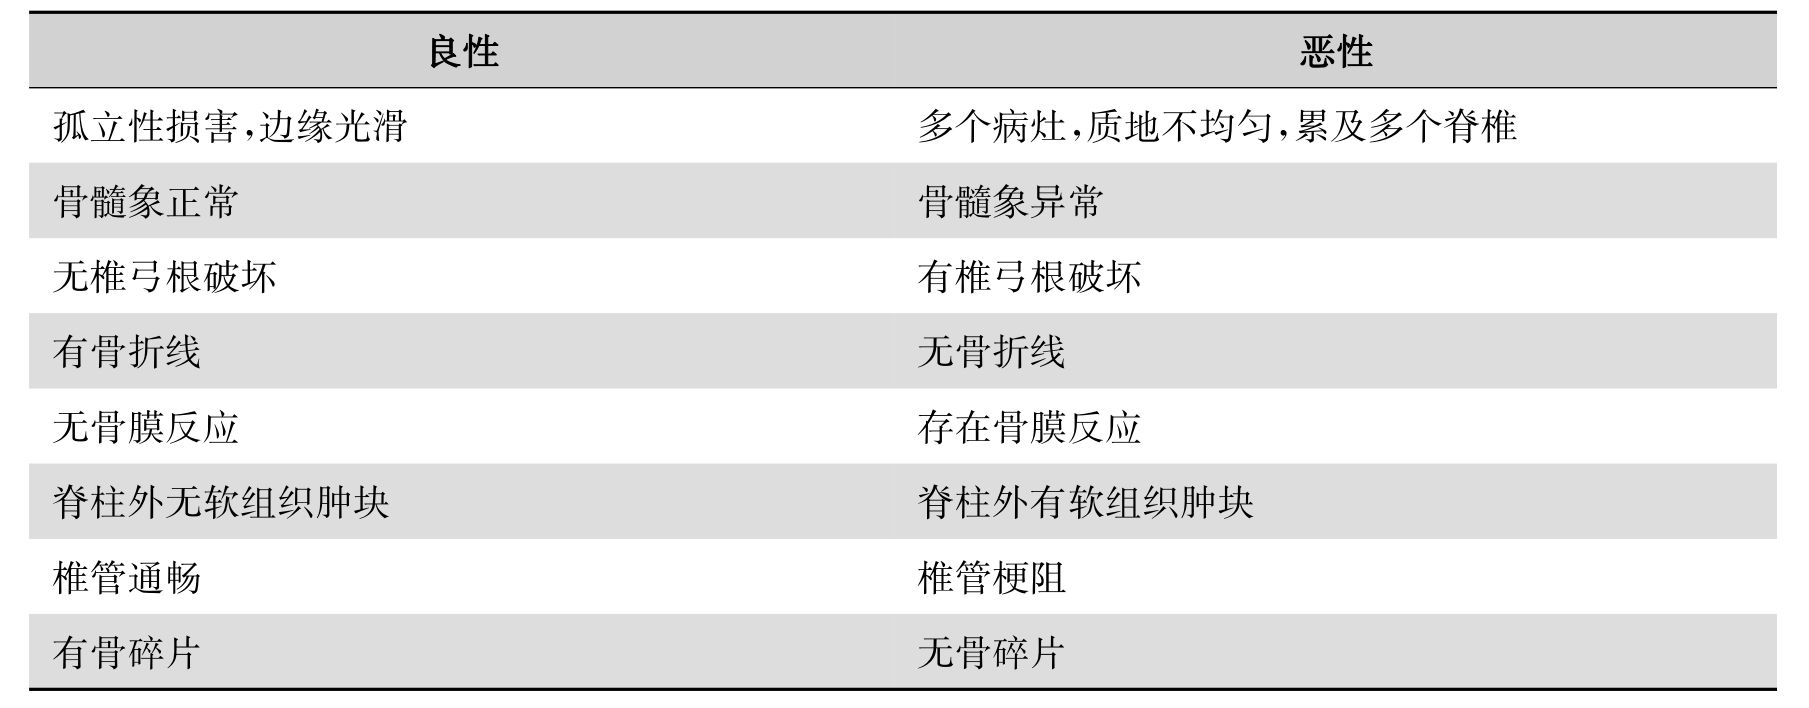
\includegraphics[width=6.02083in,height=2.34375in]{./images/Image00271.jpg}
\end{table}

\paragraph{1.多发性骨髓瘤}

多发性骨髓瘤是最常见的原发性脊柱恶性肿瘤,是由骨髓中单克隆浆细胞恶性增生所导致的疾病,克隆性浆细胞直接浸润组织和器官,导致溶骨性骨质破坏。本病多发生于老年男性。临床上几乎所有患者均有腰背痛及虚弱、体重减轻等系统症状。疼痛往往是突发性,可能是病理骨折所致。患者有贫血、血沉加快、高钙血症和肾功能不全等。一半患者尿中有尿本-周蛋白,血清蛋白固定电泳发现M蛋白。X线检查可见溶骨性破坏病灶,典型者呈穿凿样透亮缺损。骨髓穿刺和骨髓活检是确诊的重要手段。

\paragraph{2.转移性肿瘤}

脊柱是全身骨骼中最易发生骨转移的部位,脊柱转移瘤的主要原发肿瘤包括乳腺癌、肺癌、前列腺癌、卵巢癌或淋巴瘤。乳腺癌和肺癌的转移灶常见于胸椎,而前列腺癌转移灶多见于腰椎。腰椎是脊柱骨转移癌最好发的部位。脊柱转移肿瘤最常见的症状是腰背部疼痛,疼痛进行性加重,持续性钝痛,夜间加重,随着病情的进展可出现根性疼痛。神经症状常出现在病情晚期,是患者就诊的常见原因。常见运动功能减弱,其次是感觉麻木或异常,根性疼痛可以准确定位肿瘤的椎体平面。可能出现神经压迫,甚至出现截瘫、尿潴留和尿失禁。其他肿瘤相关病史,如体重减轻、食欲减退、疲乏、咯血、血尿、便血、呕血及吸烟史均有辅助作用。查体的重点是常见原发肿瘤的部位,包括乳腺、胸部、前列腺、腹部、盆腔和淋巴系统。评估脊柱转移性病变常用的影像学检查有X线平片、骨扫描、CT、MRI。只有当皮质骨破坏明显时才能被X线发现。病灶大多是溶骨性。肾上腺肿瘤、甲状腺肿瘤、大肠癌骨转移可见明显的溶骨性病灶;而乳腺癌、前列腺癌及肺癌可表现为成骨性转移。肾细胞癌骨扫描为阴性。对于年龄大于50岁,没有明显外伤的情况下出现腰背痛,卧床休息后无法缓解,突发性脊柱痉挛疼痛,ESR升高,应首先考虑恶性肿瘤,尤其对有肿瘤病史患者更应高度怀疑。

\subsection{三、炎性脊柱关节病}

脊柱关节病是一组以脊柱、骶髂及下肢关节受累为主的系统炎性疾病。包括强直性脊柱炎、银屑病关节炎、反应性关节炎、肠病性关节炎和未分化脊柱关节病。这类疾病常累及脊柱,引起腰背痛。本组疾病与HLA-B27具有较高的关联性,其腰背痛呈现出炎症性特征,以鉴别于机械性腰背痛,即:年龄小于40岁,缓慢起病,活动后疼痛减轻,休息不能缓解和夜间痛。此组疾病的疼痛对非甾体抗炎药(NSAIDs)反应较好,有助于鉴别诊断。

\subsubsection{(一)强直性脊柱炎}

强直性脊柱炎好发于年轻男性,以腰背部疼痛和僵硬为主要表现,疼痛持续存在,夜间显著,活动后症状缓解,休息时加重。随着疾病的发展,脊柱前屈和侧弯活动受限。正常的颈椎和腰椎生理性前凸消失,出现胸椎后凸畸形。可累及下肢关节,伴有附着点炎(如跟腱炎),还可出现关节外表现如虹膜炎及主动脉根部病变。实验室检查血沉和CRP可升高,90\%的患者HLA-B27阳性。X线显示骶髂关节骨质虫蚀状破坏,关节融合,椎体方形变,椎小关节模糊,椎旁韧带骨化,骨桥形成,呈“竹节样脊柱”。MRI检查对本病的早期诊断具有重要价值,可以发现骶骨和髂骨在邻近骶髂关节面附近有骨髓水肿,还可见椎体、椎弓骨髓水肿以及棘间韧带附着点炎症等表现,在压脂的T2加权像中呈现高信号。MRI增强扫描可发现骶髂关节滑膜炎,而功能超声检查对外周关节的附着点炎具有较好的诊断意义。

\subsubsection{(二)银屑病性关节炎}

银屑病性关节炎有10\%患者累及脊柱,多在20~30岁发病。银屑病皮疹是诊断本病的主要线索,但有时皮疹范围比较小或发生部位隐蔽(如骶尾部),则容易漏诊。询问病史及体检时应注意寻找有无相关的病史或皮疹。另外,大约15\%患者关节症状出现在皮疹前,增加诊断难度。银屑病性关节炎累及中轴关节时脊柱和骶髂关节的病变类似强直性脊柱炎,椎体和椎间关节炎症、侵蚀、融合、韧带骨化。体格检查表现为轴性疼痛、僵硬和活动范围变小。实验室检查血沉和CRP可升高,约20\%患者HLA-B27阳性。10\%~20\%患者血尿酸水平升高。X线显示自发的小关节融合和韧带骨赘形成,并呈不对称性。虽然银屑病性关节炎累及中轴关节时影像学检查类似强直性脊柱炎,但其程度往往比后者轻、而且病变表现为不连续性(不是所有椎体都受累)和不对称性(倾向于单侧骶髂关节受累)。此外,银屑病性关节炎的其他特征如腊肠指(近端和远端指间关节同时受累,单个手指或足趾炎症肿胀)、铅笔套征(远端指骨侵蚀)和指甲病变都有助于鉴别诊断。

\subsubsection{(三)反应性关节炎}

该病为感染后发生的反应性关节炎,最常见尿道炎和肠道感染,一般在感染后2~4周出现。本病好发于20~30岁,由性病引起的反应性关节炎男性多于女性。部分患者可有腰背痛和僵硬症状,以晨僵、静止痛,活动后改善为特点,伴有尿道炎、结膜炎、下肢寡关节炎、皮肤黏膜损害。X线上脊柱改变为非对称性椎旁骨化,呈“逗号样”骨赘形成是其特点,有跳跃性改变,骶髂关节炎为非对称性,比强直性脊柱炎的骶髂关节病变轻。

\subsubsection{(四)肠病性脊柱关节病}

继发于炎症性肠病(克罗恩病和溃疡性结肠炎)的关节炎,可有下腰痛、僵硬的表现,但患者多伴有肠道的症状如腹痛、腹泻、便秘或便血,在鉴别诊断是应注意询问相关的病史。50\%~70\%患者HLA-B27阳性。脊柱和骶髂关节的影像学发现与银屑病关节炎类似,但总体比较轻。胶囊内镜或结肠镜有助于确诊。

\subsubsection{(五)弥漫性特发性骨肥厚症(DISH)}

弥漫性特发性骨肥厚症(diffuse idiopathic skeletal
hyperostosis,DISH)并不是炎症性关节炎,但其表现容易和强直性脊柱炎混淆,为方便对比和鉴别诊断,在此一并叙述。该病主要病理改变是脊柱韧带和附着点的钙化和骨化,主要发生在椎体的前外侧,常见至少连续4个椎体韧带骨化,X线表现与强直性脊柱炎相似,但本病与HLA-B27无关,血沉和CRP等指标正常。X线上无小关节与骶髂关节的强直,椎间盘间隙存在,无椎体边缘硬化。本病多见于老年男性,常累及颈椎和低位胸椎。胸腰椎受累时,患者常表现为胸腰背部疼痛和僵硬,症状与骨赘不相关,有17\%~28\%的患者伴有吞咽困难,合并后纵韧带骨化可出现明显的脊髓受压表现。

\subsubsection{(六)髂骨致密性骨炎(osteitis condensans ilii)}

是以髂骨耳状关节部位的硬化性病变为特征。本病发病机制不明,可能是机械因素所致。本病表现容易和强直性脊柱炎混淆,但致密性骨炎一般不伴有炎症指标(血沉、CRP)的升高,没有骨质破坏或侵蚀,骶髂关节间隙正常,HLA-B27阴性。好发于妊娠后妇女(强直性脊柱炎好发于年轻男性)。患者以下腰痛为主要表现,可放射至臀部和大腿后侧,但无神经根压迫的表现,无感觉或运动神经的表现(有别于坐骨神经痛),也无全身表现。X光有特征性的表现可供鉴别诊断,即在骶髂关节的髂骨部位(骶髂关节下2/3)见边界清楚、尖端向上的三角形骨硬化区,不累及骶骨,而骶髂关节间隙正常。

\subsection{四、代谢性病变}

\subsubsection{(一)骨质疏松症}

骨质疏松症是最常见的代谢性骨骼疾病。世界卫生组织定义骨质疏松症是一种以骨量低下、骨微结构破坏,导致骨脆性增加,易发生骨折为特征的全身性骨病。骨质疏松症的危险因素包括:年龄、内分泌疾病、肿瘤、制动、缺钙饮食、酒精、低体重指数、吸烟等。类风湿关节炎、强直性脊柱炎等风湿性疾病本身及长期使用糖皮质激素均容易诱发继发性骨质疏松。骨质疏松症常无症状,但患者可发生细微的骨折,引起骨痛;出现较显著的骨折则引起剧烈疼痛。引起腰背痛的最常见骨折是椎体压缩性骨折和骶骨骨折。此时,脊柱中线深部局限性剧痛,活动或负重后加重,神经系统受累少见。双能X线吸收计量法(DEXA)是诊断骨质疏松症的金标准,一般比较严重时X线检查才能发现骨量减少。出现骨折时,X线检查可了解椎体骨折部位及程度。CT可以发现微小的骨折,高分辨率CT还能对骨质的微结构进行分析。MRI检查能显示椎管受累情况和清晰显示骨折处的骨髓水肿。骨髓水肿在T1加权像显示低信号,T2加权像显示高信号,随着时间推移,T1和T2信号逐渐恢复。MRI还能区别恶性病变。骨扫描则可灵敏地定位。血清学检查主要用于排除其他引起骨量减少的原因,如血清甲状旁腺激素、血钙、血磷和碱性磷酸酶水平等。骨形成标记如骨特异性碱性磷酸酶和骨钙素,骨吸收标记如尿中胶原降解产物(Ⅰ型胶原交联氨基末端肽和吡啶啉)有助于了解骨转运情况。

\subsubsection{(二)甲状旁腺功能亢进症}

甲状旁腺功能亢进症由于甲状旁腺大量分泌甲状旁腺激素(PTH),使骨钙溶解入血,引起高钙血症。甲状旁腺功能亢进症的患者,骨痛往往是早期唯一主诉,尤其是腰背部疼痛,症状持续性加重,久站时加重,休息后可缓解,严重时出现病理性骨折。因为长期高钙血症影响肾小管的浓缩功能,患者可出现口渴,PTH还能抑制肾小管重吸收碳酸氢盐,使尿呈碱性,容易形成尿路结石,出现肾绞痛。高钙血症患者还有疲倦、嗜睡、食欲减退和便秘等表现,高钙血症显著时因肾血管强烈收缩和脱水,可致肾功能不全。由于甲状旁腺激素能抑制肾小管上皮细胞对磷的重吸收,尿磷排泄增加,血磷降低,但在肾功能不全时血清磷可不低,尿毒症所致的继发性甲状旁腺功能亢进磷酸甚至升高。血清碱性磷酸酶增高。高钙血症、低磷血症和血清碱性磷酸酶增高是本病的主要线索,血清PTH升高是诊断原发性甲状旁腺功能亢进症的主要依据。X线检查:表现普遍性骨质疏松,弥漫性脱钙,骨密度发现骨量减少或骨质疏松症。

\subsubsection{(三)脊柱痛风}

痛风是嘌呤代谢紊乱、引起高尿酸血症,尿酸沉积在关节所引发的炎症。该病最常累及第一跖趾关节,但也可以累及任何关节,严重时累及脊柱、髋部、肩部、骶髂关节、胸锁关节和肩锁关节等。累及脊柱或骶髂关节时,表现腰背部疼痛,可以是持续慢性钝痛,也可以是急性发作性剧痛,伴或不伴有神经根痛。尿酸盐可沉积在腰椎椎弓根、椎板和黄韧带。脊柱痛风石或滑膜囊肿可导致椎管狭窄,引起神经性跛行。影像学检查发现因尿酸盐沉积侵蚀椎骨,导致骨质破坏和硬化。脊柱近关节区或关节内形成软组织团块影,密度高于周围软组织,边界清楚,周围有钙化,可压迫脊髓或马尾神经。CT上表现类似炎症或肿瘤。MRI有助于鉴别诊断,在T2加权像中表现为低密度影,周围有纤维组织包绕。不过,增强对比时,痛风石也可强化,这与炎症和肿瘤比较难区别。出现脊柱痛风者,往往病情十分显著,有多年高尿酸血症和反复痛风发作病史,全身多关节受累、畸形并有多处痛风石形成;结合影像学检查,比较容易进行鉴别诊断。

\subsection{五、变形性骨炎(Paget病)}

变形性骨炎,多见中老年男性,病因不明。本病主要病理改变是老化的骨骼局部骨代谢异常,骨转运加速,破骨和成骨过程紊乱,导致局部骨增大、变形,主要累及颅骨、脊柱、骨盆和下肢长骨。发生在脊柱时,腰椎、骶椎好发,尤其是L\textsubscript{4}
、L\textsubscript{5}
椎体,表现为局限性的腰背痛,出现驼背。血清碱性磷酸酶显著升高,但血钙和血磷一般正常。X线表现同时可见破骨和成骨过程,表现为局限性的密度降低和增加同时存在,骨皮质增厚、骨小梁增粗紊乱,椎体增大、变形、密度增高。椎体周边硬化或镜框状椎体是Paget病的特征性表现,椎体和椎弓均可受累。

\subsection{六、舒尔曼脊柱后凸(Scheuermann脊柱后凸)}

舒尔曼脊柱后凸具有很强遗传倾向,为常染色体显性遗传,症状在10~14岁之间逐渐显现,男性偏多。有研究认为,钙离子代谢异常和所引起的骨质疏松是椎体楔形变的主要原因。早期背痛比较轻微,骨骼发育成熟后腰背痛症状加重,成年仍有背痛,主要表现为严重的脊柱后凸。患者常伴有腘绳肌紧缩感,造成骨盆后倾,躯干向后合力增加导致脊柱要前屈来保持躯体矢状面的平衡。舒尔曼脊柱后凸还可伴有其他疾病,包括内分泌异常、维生素缺乏、感染、神经肌肉病变,但这些疾病和本病没有直接的因果关系。体格检查注意皮肤有无褐色斑和腋窝、腹股沟斑点(提示多发性神经纤维瘤)。X线特征包括椎体楔形变和终板不规则。

\subsection{七、镰状细胞性贫血}

镰状细胞性贫血又称纯合子型镰状细胞血红蛋白病。本病是血红蛋白β链第6位上的谷氨酸被缬氨酸替代后形成血红蛋白S。在缺氧条件下,血红蛋白S聚合成细长结晶,使红细胞变成镰状。镰状红细胞僵硬、变形性差,难于通过毛细血管,阻塞毛细血管,导致临床上出现溶血性贫血和血栓形成。在发生镰状细胞梗死型(疼痛型)危象时,可出现腰背痛和腿部疼痛,容易误诊为骨骼系统疾病。本病的诊断依据:①贫血,黄疸,网织红细胞增多;②腹痛和腿痛;③脾脏早期可肿大,但后期不大(多次脾梗死形成的瘢痕组织收缩使脾脏缩小);④溶血危象;⑤镰变试验(sickling
test)阳性;⑥血红蛋白电泳主要成分为血红蛋白S。

\subsection{八、蛛网膜下腔出血}

蛛网膜下腔出血的病因包括:颅内动脉瘤、脑动静脉畸形、高血压脑动脉硬化和烟雾病等。由动脉瘤破裂所致多见,好发于30~60岁,女性多于男性,血管畸形多见青少年。发病前常无先兆,患者突然出现剧烈头痛、烦躁、脑膜刺激征与血性脑脊液,开始时仅有剧烈头痛、颈项痛,蛛网膜下腔血液向下流刺激脊膜和脊神经根,可致剧烈的腰背痛和下肢痛。绝大多数病例发病数小时出现脑膜刺激征,以颈项强直最为明显,Kernig征、Brudzinski征阳性。意识障碍与出血量有关,一般神志清楚,也可有不同程度意识障碍。少数患者急性期出现精神症状,如欣快、谵妄、幻觉等,2~3周后自然消失。约有25\%患者眼科检查可见玻璃体下片状出血,发病1小时内可出现,有诊断特异性。

\protect\hypertarget{text00335.html}{}{}

\section{147 内脏疾病}

\subsection{一、盆腔疾病}

\subsubsection{(一)前列腺炎}

此病多见于30~40岁的男性,常与慢性精囊炎同时存在。主要症状为腰痛、会阴部不适感、尿道灼热感、尿频和神经衰弱症状。检查前列腺液发现白细胞增多、卵磷脂减少。

\subsubsection{(二)子宫内膜异位症}

腰骶部或下腹部阴道疼痛,常在月经来潮前出现,月经期持续疼痛,少数在月经干净后可以加重。伴有月经失调、月经量过多和性交痛。月经前出现恶心、呕吐。

\subsubsection{(三)慢性盆腔炎}

下腹部或腰部隐痛或明显疼痛,月经周期不规则,闭经或偶尔月经量非常多,白带有异味,有大量的阴道分泌物,时常出现尿痛,食欲下降,伴有恶心呕吐。

\subsection{二、腹膜后疾病}

\subsubsection{(一)肾脏和肾上腺疾病}

\paragraph{1.肾结石}

主要症状是疼痛和血尿,疼痛一般为腰部肾区或上腹部的钝痛、隐痛或绞痛,为阵发性,常突然发生,刀割样痛,可经下腹部放射到大腿内侧,有时伴有恶心、呕吐,面色苍白,脉搏细弱,血压下降。血尿多出现活动或剧烈绞痛后发生。伴有尿频、尿急、尿痛等,合并感染时可出现发热。

\paragraph{2.肾盂肾炎}

肾盂肾炎常有腰部酸痛,慢性期无尿路刺激征或症状较轻,临床上容易误诊;急性期常有明显的尿路刺激症状、脓尿,并伴有寒战、发热、白细胞增高等细菌感染的表现。

\paragraph{3.肾周脓肿}

肾周脓肿常伴有腰部胀痛,弯腰时疼痛症状明显加重,可出现腰部痛性肿块。患者常有全身严重感染的表现。CT或MRI检查有助于明确诊断。

\paragraph{4.慢性肾小球肾炎}

部分慢性肾小球肾炎患者诉有腰痛,特别是IgA肾病患者,原因未明。患者常有血尿、蛋白尿、管型尿、高血压和肾功能不全。尿红细胞位相检查发现畸形红细胞,肾活检有助于明确诊断。

\paragraph{5.肾上腺和腹膜后疾病}

肾上腺肿瘤和或腹膜后肿瘤常导致腰背痛,多为持续性胀痛或钝痛。腹膜后肿瘤以淋巴瘤多见。腹膜后纤维化也压迫输尿管等结构而引起腰背痛。

\subsubsection{(二)主动脉瘤}

胸腹主动脉瘤可出现腰背部疼痛,尤其当动脉瘤破裂形成主动脉夹层时,患者表现为突发性腰背部剧烈疼痛,多见于有高血压史的老年人,应注意鉴别诊断。

\subsubsection{(三)胰腺疾病}

\paragraph{1.急性胰腺炎}

可出现左背部放射性痛,胰腺的痛觉神经也可由内脏神经纤维束传至第6~11胸神经节,该神经节为双侧性,因此急性胰腺炎急腹症常向左侧腰背部神经放射。

\paragraph{2.胰腺癌}

尤其是腺体和尾部肿瘤,常有顽固性难忍的腰背部疼痛,患者夜间不能入睡,不能平卧,疼痛在脊柱屈曲时减轻、坐位时感到舒适。患者常有黄疸、消瘦和衰竭。

\subsection{三、腹腔疾病}

\subsubsection{(一)胆囊炎}

可因刺激膈神经末梢而产生左肩背部疼痛,但这类患者同时可伴有右上腹胆囊区压痛。

\subsubsection{(二)消化系统溃疡}

胃及十二指肠溃疡患者,可表现为胸背部的疼痛,疼痛偏左侧,在同一区域可查及压痛点,穿透性溃疡有明显疼痛,非穿透性溃疡也可有背部放射痛,尤其是十二指肠球后溃疡,患者通常已有消化系统的症状,有时伴有上腹部疼痛,疼痛与脊柱活动无关。

\protect\hypertarget{text00336.html}{}{}

\section{148 其他腰背痛}

即使有上述多种病因,还有一些腰背痛的确切病因并不清楚,这些腰背痛可以归入其他腰背痛。其疼痛程度一般并不严重,无严重的基础疾病,预后良好,可以给予一般对症处理即可。部分腰背痛还与患者精神因素有关,如纤维肌痛综合征,患者可出现广泛性疼痛,腰背部疼痛比较常见,疼痛性质多样,疼痛程度时轻时重,休息常不能缓解,常伴有疲劳、睡眠障碍以及抑郁和焦虑等精神症状;还有躯体化障碍的患者,常常有多种多样、反复出现,经常变化的躯体症状为主,患者主诉较多,可有腰背痛和胸痛的症状,体检和实验室检查不能发现躯体障碍的证据,但患者痛苦,不断求诊,和独居、接受外界刺激较少、抑郁和焦虑情绪相关。对于这些患者应注意适当从精神上给予支持或治疗。

\protect\hypertarget{text00337.html}{}{}

\section{参考文献}

1.孙凌云,Trotta F.骨Paget病.风湿病学杂志,1997,2(4):25-29

2.黄光,刘兴洲.Paget骨病的临床特点及其诊治.中国全科医学,2008,11(18):1658-1659

3.周辅昔,王绍武.镰状细胞性贫血儿童疼痛性骨危象的Gd-DOTA增强MRI.国外医学(临床放射学分册),1995,10(5):309

4.于洪炜.腰背痛.社区医学杂志,2007,5(12):21-23

5.何晓清,徐永清,朱跃良.腰背痛流行病学进展.国际骨科学杂志,2008,29(2):115-116

6.戴力扬.腰背痛的流行病学.颈腰痛杂志,2000,21(2):162-164

7.周伟.儿童腰背痛.颈腰痛杂志,1999,20(1):73-75

8.金克峙.职业性腰背痛的流行病学研究.劳动医学,1999,16(1):53-55

9.段红光.颈肩腰背痛.中国全科医学,2006,9(12):969-970

10.李钦亮,马迅.儿童腰背痛.实用骨科杂志,2003,9(2):142-145

11.孟卫平,陈永林.老年人腰背痛的病因及鉴别诊断.中国误诊学杂志,2001,1(3):460-462

12.韩焱,等.青年女性慢性非特异性腰背痛椎旁肌变化的CT表现.颈腰背痛杂志,2010,31(2):83-85

13.姜召彩,苏园林.腰背痛.中国疼痛医学杂志,2010,16(6):321-323

14.许岳俊,陈佩珊,詹旋燕.以腰背痛为首发症状的胰腺癌11例.罕少疾病杂志,2006,13(2):38-39

15.李志刚.谈腰背痛与椎间盘疾病.中国现代药物应用,2008,2(5):86

16.金文杰,戴力扬.肌肉疲劳与慢性腰背痛.颈腰痛杂志,2004,25(2):134-136

17.张铁超,侯树勋,姚长海.年轻女性慢性腰背痛.中国脊柱脊髓杂志,2004,14(12):760

18.张铁超,侯树勋,姚长海.年轻女性慢性腰背痛(续).中国脊柱脊髓杂志,2005,15(1):37

19.白玉贞,韩晓东,牛广明.布氏杆菌性脊椎炎的MRI表现.临床放射学杂志,2012,31(1):96-100

20.曹吉怀,等.布鲁菌病脊柱炎与脊柱结核的CT及MRI鉴别诊断.放射学实践,2013,28(2):196-199

21.盛伟斌,等.脊柱包虫病的临床特点及诊断方法.中华骨科杂志,2006,26(1):7-12

22.宋兴华,等.评估X、CT及MRI在脊柱包虫病诊断中的价值.颈腰痛杂志,2007,28(6):469-472

23.韩国伟,等.真菌性脊柱炎1例报告.中国矫形外科杂志,2003,11(13):873

24.文泽军,等.脊柱嗜酸性肉芽肿的影像学诊断.放射学实践,2007,22(7):737-739

25.朱勇,等.脊柱嗜酸性肉芽肿的诊断及治疗.中国现代医学杂志,2005,15(18):2828-2829

26.桂斌捷,等.青少年和成人脊柱嗜酸性肉芽肿的影像学表现.临床骨科杂志,2005,8(5):385-387

27.颜华东,等.脊柱嗜酸性肉芽肿诊断与治疗.国际骨科学杂志,2013,17(2):88-90

28.马庆军,等.脊柱骨巨细胞瘤36例诊断与治疗.北京大学学报(医学版),2002,34(6):656-659

29.杜联军,等.脊柱骨巨细胞瘤的影像学表现及临床意义.实用放射学杂志,2006,22(3):300-303

30.常恒,王俭,肖湘生.脊柱骨巨细胞瘤的影像学诊断.临床放射学杂志,2003,22(1):55-57

31.贾连顺.弥漫性特发性骨肥厚症的概念与临床特征.中国矫形外科杂志,2007,15(17):1319-1321

32.顾雪梅,李珍平.弥漫性特发性骨肥厚症的临床及影像学特点.中国全科医学,2008,11(3):257

33.刘悦震,史朝瑞.致密性骨炎的骶髂关节CT表现(附40例分析).现代医用影像学,2009,18(2):126-127

34.李盛华,等.骶髂关节致密性骨炎诊疗指南编写报告.全国第七次中国整脊学学术交流大会,2011,35

35.韩乙庭.脊柱痛风.河南医药信息,1997,5(4):57-58

36.DavidA Wong,Ensor
Transfeldt.麦氏腰背痛.第4版.谭军,郝定均译.北京:人民军医出版社,2009

37.Bono GM,Garfin
SR.骨科必备丛书(脊柱).雷伟,孙宏慧译.西安:第四军医大学出版社,2008

38.段承祥.脊柱影像学.北京:化学工业出版社,2007

39.Siemionow K,et al.Identifying serious causes of back
pain:cancer,infection,fracture.Cleve Clin J
Med,2008,75(8):557-566

40.Haswell K,Gilmour J,Moore B.Clinical decision rules for
identification of low back pain patients with neurologic involvement in
primary care.Spine(Phila Pa 1976),2008,33(1):68-73

41.Roudsari B,Jarvik JG.Lumbar spine MRI for low back pain:indications
and yield.AJR Am J Roentgenol,2010,195(3):550-559

42.Wilson JF.In the clinic.Low back pain.Ann Intern
Med,2008,148(9):ITC5-1-ITC5-16

43.Manusov EG.Evaluation and diagnosis of low back pain.Prim
Care,2012,39(9):471-479

44.Kaufmann JA.Low back pain:diagnosis and management in primary
care.Lippincotts Prim Care Pract,1999,3(4):376-393

45.Koes BW,et al.An updated overview of clinical guidelines for the
management of non-specific low back pain in primary care.Eur Spine
J,2010,19(12):2075-2094

46.Gerr F,Mani L.Work-related low back pain.Prim
Care,2000,27(4):865-876

47.Indahl A.Low back pain:diagnosis,treatment,and prognosis.Scand J
Rheumatol,2004,33:199-209

\protect\hypertarget{text00338.html}{}{}

